% Kelpod status-update slides (Frontier Systems, WiSe 2026/2027).
% Build:   make slides    -> pdf/kelpod-slides.pdf    (one page per click; presenting from PDF)
%          make handout   -> pdf/kelpod-handout.pdf   (one page per slide, final state)
%          make notes     -> pdf/kelpod-notes.pdf     (slides + speaker notes, 2 per page)
% Animations are appear-only: \uncover<n-> keeps the space, so nothing moves between clicks.
% Speaker notes live in \note{...}.

\ifdefined\SHOWNOTES
  \documentclass[aspectratio=169,notes=show]{beamer}
  \usepackage{pgfpages}
  \pgfpagesuselayout{2 on 1}[a4paper,landscape,border shrink=5mm]
\else\ifdefined\HANDOUT
  \documentclass[aspectratio=169,handout]{beamer}
\else
  \documentclass[aspectratio=169]{beamer}
\fi\fi

\usepackage{graphicx}
\usepackage{tikz}
\usetikzlibrary{positioning,arrows.meta}

% --- Colours: same palette as the earlier Kelpod and skill-following decks ------
\definecolor{kblue}{HTML}{3333B2}
\definecolor{kbluedark}{HTML}{26268A}
\definecolor{kred}{HTML}{C62828}
\definecolor{kgreen}{HTML}{2E7D32}
\definecolor{kgrey}{HTML}{555566}
\definecolor{kpale}{HTML}{E6E6F6}

\usetheme{Madrid}
\setbeamercolor{structure}{fg=kblue}
\setbeamercolor{palette primary}{bg=kblue,fg=white}
\setbeamercolor{palette secondary}{bg=kbluedark,fg=white}
\setbeamercolor{palette tertiary}{bg=kbluedark,fg=white}
\setbeamercolor{title}{fg=white}
\setbeamercolor{subtitle}{fg=white}
\setbeamercolor{author}{fg=black}
\setbeamercolor{frametitle}{bg=kblue,fg=white}
\setbeamercolor{block title}{bg=kblue,fg=white}
\setbeamercolor{block body}{bg=kblue!12,fg=black}
\setbeamercolor{block title alerted}{bg=kred,fg=white}
\setbeamercolor{block body alerted}{bg=kred!12,fg=black}
\setbeamercolor{block title example}{bg=kgreen,fg=white}
\setbeamercolor{block body example}{bg=kgreen!12,fg=black}
\setbeamercolor{alerted text}{fg=kred}
\setbeamercolor{example text}{fg=kgreen}
\setbeamertemplate{navigation symbols}{}
\setbeamertemplate{blocks}[rounded][shadow=false]
\setbeamertemplate{itemize items}[triangle]
\setbeamercolor{itemize item}{fg=kblue}
\setbeamercolor{itemize subitem}{fg=kblue}
\setbeamerfont{block title}{series=\bfseries}

% Shared look for diagram boxes
\tikzset{
  box/.style={draw=kblue, very thick, rounded corners, fill=kpale, align=center,
              minimum height=1.0cm, font=\small},
  arr/.style={-{Stealth[length=2.2mm]}, very thick, kblue},
  tile/.style={draw=kblue, very thick, rounded corners, fill=white, align=center,
               minimum width=3.6cm, minimum height=1.9cm},
}

\title[Kelpod]{Kelpod}
\subtitle{Old floor plans to energy-ready 3D models}
\author[Tajdeen \& Antony]{Arsha Fahima Tajdeen \and Kevin Antony}
\institute[Frontier Systems]{Frontier Systems, WiSe 2026/2027}
\date{}

\begin{document}
\begin{frame}[plain]
  \titlepage
  \note{Hi everyone. We are Arsha and Kevin, and this is Kelpod. We turn old building plans into 3D
  models that energy software can use.}
\end{frame}

% ---------------------------------------------------------------------------
\begin{frame}{The problem}
  \begin{columns}[T,onlytextwidth]
    \column{0.56\textwidth}
      \begin{itemize}
        \item<2-> GEG: millions of buildings need energy audits
        \item<3-> Most only have old PDF scans
        \item<4-> Experts redraw each plan in HottCAD: 3--6 h
      \end{itemize}
    \column{0.40\textwidth}
      \centering
      
\includegraphics[height=0.50\textheight,keepaspectratio]{images/multifamily-house-saxony.jpg}\\[3pt]
      {\tiny Photo: August Geyler, \mbox{CC BY-SA 4.0} (Wikimedia Commons)}
  \end{columns}
  \note{Germany has to renovate a huge number of old buildings, like this one in Saxony.
  [click] The building energy law means millions of them need an energy audit.
  [click] But most old buildings only have old PDF scans of their plans.
  [click] So an energy expert redraws every plan by hand in HottCAD, the standard energy software. That
  takes three to six hours, before the real work even starts.}
\end{frame}

% ---------------------------------------------------------------------------
\begin{frame}{Today's AI can't do it}
  \begin{itemize}
    \item<2-> DeepFloorPlan, RoomFormer: trained on US plans
    \item<3-> Can't read DIN 1356-1
    \item<4-> Output: pixel masks, not vector models
  \end{itemize}
  \note{Why not just use AI?
  [click] The existing floor-plan models were trained on American plans.
  [click] German plans follow their own drawing standard, and those models misread it.
  [click] And they only give you a coloured picture. Energy software needs a real model with closed walls
  and rooms.}
\end{frame}

% ---------------------------------------------------------------------------
\begin{frame}{Kelpod: old plan in, 3D model out}
  \begin{center}
  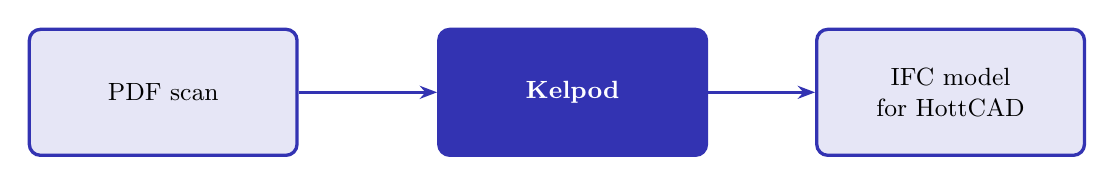
\begin{tikzpicture}
    \node[box, minimum width=3.4cm, minimum height=1.6cm] (in) at (0,0) {PDF scan};
    \node<2->[box, minimum width=3.4cm, minimum height=1.6cm, fill=kblue, text=white] (k) at (5.2,0) {\textbf{Kelpod}};
    \node<3->[box, minimum width=3.4cm, minimum height=1.6cm] (out) at (10.0,0) {IFC model\\for HottCAD};
    \draw<2->[arr] (in) -- (k);
    \draw<3->[arr] (k) -- (out);
  \end{tikzpicture}
  \end{center}
  \vspace{0.8em}
  \uncover<4->{\begin{center}\Large Under 3 minutes instead of 3--6 hours\end{center}}
  \note{That's what Kelpod does. You give it the old scan.
  [click] Kelpod reads it.
  [click] And produces a 3D model in IFC, the standard building-model format, which HottCAD opens directly.
  [click] Our goal is under three minutes per plan instead of three to six hours. The expert only checks
  the result.}
\end{frame}

% ---------------------------------------------------------------------------
\begin{frame}{How it works}
  \begin{center}
  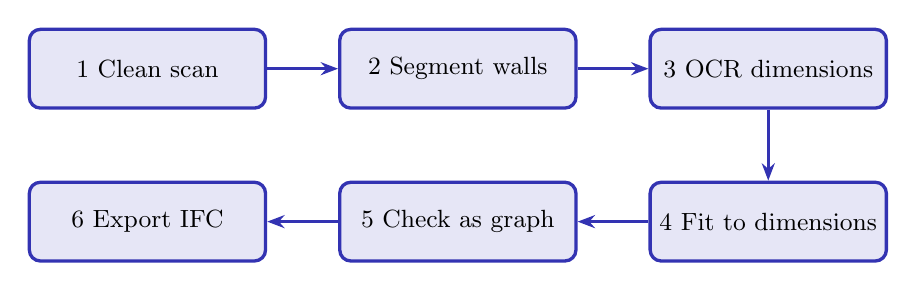
\begin{tikzpicture}[node distance=0.9cm and 0.9cm,
      stage/.style={box, minimum width=3.0cm, font=\small}]
    \node[stage] (a) {1 Clean scan};
    \node<2->[stage, right=of a] (b) {2 Segment walls};
    \node<3->[stage, right=of b] (c) {3 OCR dimensions};
    \node<4->[stage, below=of c] (d) {4 Fit to dimensions};
    \node<5->[stage, left=of d] (e) {5 Check as graph};
    \node<6->[stage, left=of e] (f) {6 Export IFC};
    \draw<2->[arr] (a) -- (b);
    \draw<3->[arr] (b) -- (c);
    \draw<4->[arr] (c) -- (d);
    \draw<5->[arr] (d) -- (e);
    \draw<6->[arr] (e) -- (f);
  \end{tikzpicture}
  \end{center}
  \note{Six steps. We clean the scan.
  [click] Find the walls, doors and windows.
  [click] Read the measurements written on the plan.
  [click] Move the walls so they match those measurements, because the drawing itself is often slightly off.
  [click] Check that everything connects: no gaps, every room closed.
  [click] And export the 3D model.}
\end{frame}

% ---------------------------------------------------------------------------
\begin{frame}{Integrate first, then replace}
  \begin{center}
  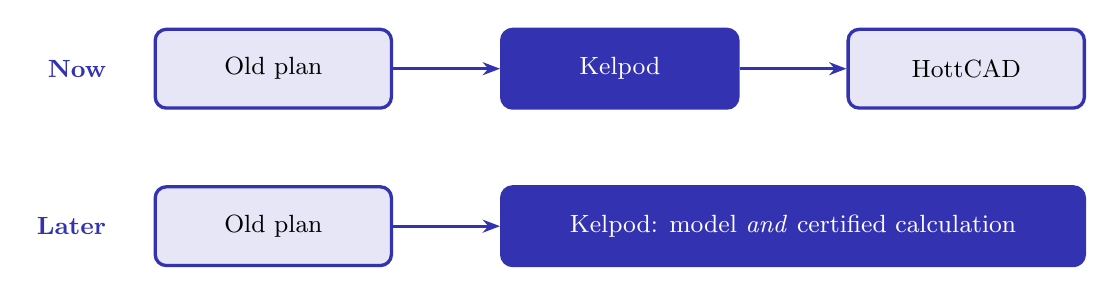
\begin{tikzpicture}
    \node[font=\bfseries\small, kblue, anchor=east] at (-2.0,0) {Now};
    \node[box, minimum width=3.0cm] (p1) at (0,0) {Old plan};
    \node<2->[box, minimum width=3.0cm, fill=kblue, text=white] (k1) at (4.4,0) {Kelpod};
    \node<2->[box, minimum width=3.0cm] (h1) at (8.8,0) {HottCAD};
    \draw<2->[arr] (p1) -- (k1);
    \draw<2->[arr] (k1) -- (h1);
    \node<3->[font=\bfseries\small, kblue, anchor=east] at (-2.0,-2.0) {Later};
    \node<3->[box, minimum width=3.0cm] (p2) at (0,-2.0) {Old plan};
    \node<3->[box, minimum width=7.4cm, fill=kblue, text=white] (k2) at (6.6,-2.0) {Kelpod: model \emph{and} certified calculation};
    \draw<3->[arr] (p2) -- (k2);
  \end{tikzpicture}
  \end{center}
  \note{Our strategy has two phases. Today the expert starts from an old plan.
  [click] Kelpod builds the model, and it goes into HottCAD for the official calculation. That saves hours
  and earns us trust and real data.
  [click] Later, Kelpod does the official calculation itself, and the expert no longer needs HottCAD. That
  needs a certified calculation engine, so we start with the part we can win now.}
\end{frame}

% ---------------------------------------------------------------------------
\begin{frame}{Customers and revenue}
  \begin{columns}[T,onlytextwidth]
    \column{0.48\textwidth}
      \begin{block}{Customers}
        Energy experts (EEE)\\
        Surveyors, architects\\
        Housing companies
      \end{block}
    \column{0.48\textwidth}
      \uncover<2->{\begin{block}{Revenue}
        30--80 EUR per plan\\
        Monthly licence\\
        API / white-label
      \end{block}}
  \end{columns}
  \note{Who pays? Energy-efficiency experts, surveyors, architects, and housing companies with thousands of
  flats.
  [click] We charge 30 to 80 euros per plan, or a monthly licence, and larger clients can build Kelpod into
  their own software.}
\end{frame}

% ---------------------------------------------------------------------------
\begin{frame}{Traction and roadmap}
  \begin{exampleblock}{1 pilot customer locked in}
  \end{exampleblock}
  \vspace{0.8em}
  \begin{center}
  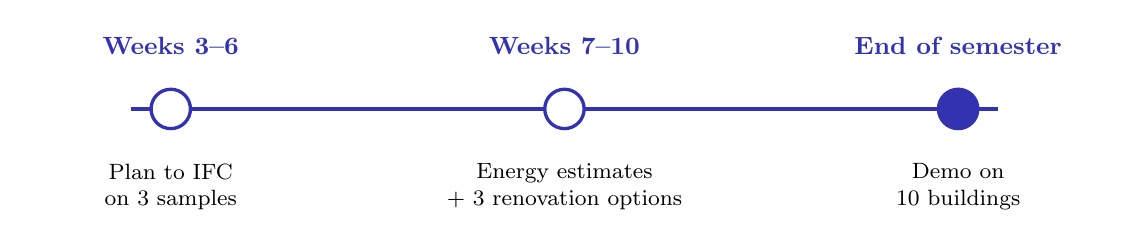
\begin{tikzpicture}
    \draw[very thick, kblue] (0,0) -- (11,0);
    \node[circle, draw=kblue, very thick, fill=white, minimum size=5mm, inner sep=0pt] (m1) at (0.5,0) {};
    \node[circle, draw=kblue, very thick, fill=white, minimum size=5mm, inner sep=0pt] (m2) at (5.5,0) {};
    \node[circle, draw=kblue, very thick, fill=kblue, minimum size=5mm, inner sep=0pt] (m3) at (10.5,0) {};
    \node[above=3mm of m1, font=\bfseries\small, kblue] {Weeks 3--6};
    \node[above=3mm of m2, font=\bfseries\small, kblue] {Weeks 7--10};
    \node[above=3mm of m3, font=\bfseries\small, kblue] {End of semester};
    \node<2->[below=3mm of m1, align=center, font=\footnotesize, text width=3.4cm] {Plan to IFC\\on 3 samples};
    \node<3->[below=3mm of m2, align=center, font=\footnotesize, text width=3.4cm] {Energy estimates\\+ 3 renovation options};
    \node<4->[below=3mm of m3, align=center, font=\footnotesize, text width=3.4cm] {Demo on\\10 buildings};
  \end{tikzpicture}
  \end{center}
  \note{One pilot customer is locked in: an energy expert. They get Kelpod for free, and we get real plans
  and feedback. We build the company with AI agents too: coding, research and sales agents, with the
  founders making the decisions.
  [click] By week 6: plan to IFC model on three sample plans.
  [click] By week 10: energy estimates and three renovation options per building.
  [click] By the end of the semester: a demo on ten buildings. Thank you, we are happy to take questions.}
\end{frame}

\end{document}
